\begin{block}{提案手法:条件付き確率場による単純型付け}
  (同一変数の頂点をマージした)型注釈付き AST に\\点数を付ける\\
  \structure{具体例}:$\lambda x. \IF~x~\THEN~\FALSE~\ELSE~\TRUE$
  \begin{itemize}
  \item 因子ノード(黒い四角)ごとに点数を計算
  \item \alert{合計点数が最大}となる型注釈の割り当て方が正解\\(の可能性が高い)
  \end{itemize}
  \vskip1em
  \begin{beamercolorbox}{figure}
    \raggedleft
    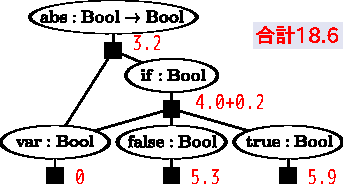
\includegraphics[height=18cm]{crf-typing-score1.pdf}
  \end{beamercolorbox}
  \vskip0.5\baselineskip
  \begin{beamercolorbox}{figure}
    \raggedleft
    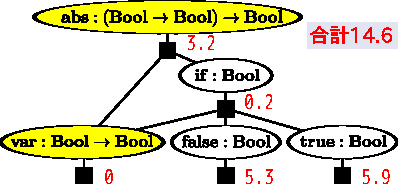
\includegraphics[height=18cm]{crf-typing-score2.pdf}
  \end{beamercolorbox}
  \vskip1em
  \begin{table}
    \centering
    \begin{tabular}{l@{\hskip1ex}r@{\hskip6ex}l@{\hskip1ex}r}\hline
      特徴{\small(型付け規則)} & 重み & 特徴{\small(型付け規則)} & 重み \\\hline
      \textsc{T-True} & 5.9 & \textsc{T-False} & 5.3 \\
      \textsc{T-Abs} & 3.2 & \textsc{T-App} & 1.7 \\
      \textsc{T-If} & 4.0 & \textsc{T-WeakIf1} & 0.2 \\\hline
    \end{tabular}
    \caption{\normalsize{}点数表}
  \end{table}
\end{block}